\section{Evaluation}
\subsection{Techniques used in the evaluation}
For the statistical evaluation of the measurements we relied on the \textit{python} programming language~
\cite{python} with several packages, including \textit{matplotlib}~\cite{Hunter2007} for plotting,
 \textit{scipy}~\cite{scipy} for fitting and \textit{uncertainties}~\cite{uc} for error propagation. 
The fitted lines
were done in each case with a least-square fit of the respective distribution. The uncertainty of each fit
is given by its covariance matrix, which we will give for each fit since it is not unlikely that the parameters
correlate. Further calculations are always done using those covariance matrices. Lets assume we have random
variables $x_0,...,x_N$ which are correlatated through the $N\times N$ Matrix $cov(x_i,x_j)$, respectively.
Further we assume to have a skalar function $f(x_0,...,x_N) \rightarrow \mathbb{R}$, then the variance
of this new random variable can be estimated (linearly) by:
\begin{equation}
Var[f] = \sigma^2 = \sum_{i,j} \frac{\partial f}{\partial x_i} \frac{\partial f}{\partial x_j} cov(x_i,x_j)
\end{equation} 
This is implicitly done within each calculation which is applied in our evaluation (we will not emphasize this
procedure in every calculation). If not further specified, we suppose that we can apply a poisson distribution
for each bin, such that the error we use is $\mu = \sqrt{N}$ like a poisson process would predict.
\subsection{Energy spectrum}
The first step in the evaluation is to make sure that the peaks which are used can be related
to the events we are looking for in the right energy scale.
In order to relate the channels to
 energies we first use fits for the different peaks in order
to fit these peaks linearly (see figure~\ref{fig:fit_peaks}). 

\begin{align*}
    A_1 &=& \left(6.7 \pm 5.4\right) \times 10^{2} \quad \mathrm{counts}\\
    A_2 &=& \left(7.95 \pm 0.29\right) \times 10^{3} \quad\mathrm{counts}\\
    A_3 &=& \left(2.16 \pm 0.04\right) \times 10^{4} \quad\mathrm{counts}\\
    \mu_1 &=& 22.4 \pm 0.4 \quad\mathrm{channels}\\
    \mu_2 &=& 45.24 \pm 0.21 \quad\mathrm{channels}\\
    \mu_3 &=& 95.74 \pm 0.14 \quad\mathrm{channels}\\
    \sigma_1 &=& -0.4 \pm 0.4 \quad\mathrm{channels}\\
    \sigma_2 &=& 4.54 \pm 0.13 \quad\mathrm{channels}\\
    \sigma_3 &=& 6.61 \pm 0.08 \quad\mathrm{channels}\\
    c &=& 827.0 \pm 21.6\quad \mathrm{counts}
\end{align*}
\begin{figure}[htpb]
    \centering
    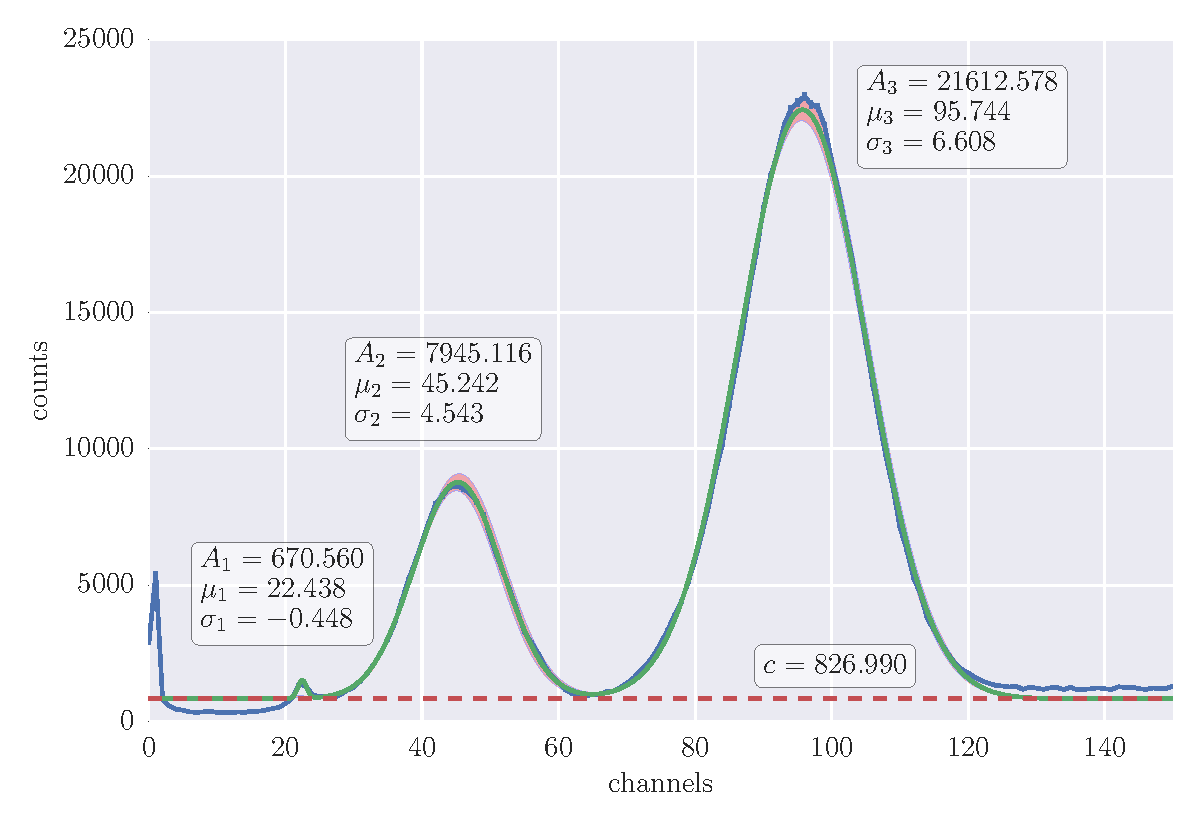
\includegraphics[width=1.1\linewidth]{analysis/figures/plot6_3_reg}
    \caption{These are the fitting curves of the americium spectrum with respect to gaussian distributions. The covariance matrix
        is given in section~\ref{subs:covariance}, along with the parameters and their errors.
        $A_1\exp{\left[\frac{(x-\mu_1)^2}{2 \sigma_1^2} \right]}+
         A_2\exp{\left[\frac{(x-\mu_2)^2}{2 \sigma_2^2} \right]}+
         A_3\exp{\left[\frac{(x-\mu_3)^2}{2 \sigma_3^2} \right]}+ c$}
        The measured data is plotted in blue, the fits are shown in green with corresponding 
        errors underlying. 
         \label{fig:fit1}
\end{figure}

\begin{align*}
    A_1 &=& \left(3.6 \pm 1.2\right) \times 10^{2} \quad \mathrm{counts}\\
    A_2 &=& \left(2.555 \pm 0.030\right) \times 10^{4} \quad \mathrm{counts}\\
    \mu_1 &=& 18.2 \pm 0.8 \quad \mathrm{channels}\\
    \mu_2 &=& 193.76 \pm 0.13 \quad \mathrm{channels}\\
    \sigma_1 &=& 1.7 \pm 0.6 \quad \mathrm{channels}\\
    \sigma_2 &=& 8.33 \pm 0.08 \quad \mathrm{channels}\\
    c &=& 124.6 \pm 16.5 \quad \mathrm{counts}
\end{align*}


\begin{figure}[htpb]
    \centering
    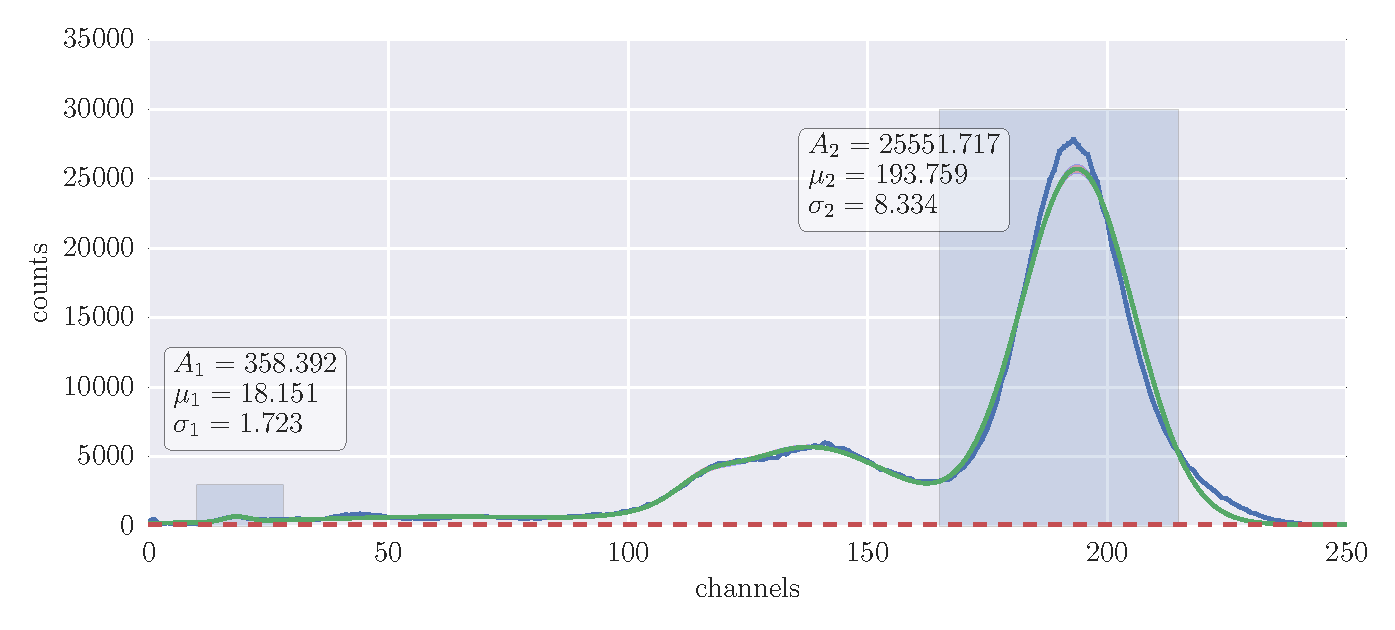
\includegraphics[width=1.1\linewidth]{analysis/figures/plot2_1a_reg}
    \caption{These are the fitting curves of the cobalt spectrum with respect to gaussian distributions:
        $A_1\exp{\left[\frac{(x-\mu_1)^2}{2 \sigma_1^2} \right]}+
         A_2\exp{\left[\frac{(x-\mu_2)^2}{2 \sigma_2^2} \right]}+
         A_3\exp{\left[\frac{(x-\mu_3)^2}{2 \sigma_3^2} \right]}+ 
         A_4\exp{\left[\frac{(x-\mu_4)^2}{2 \sigma_4^2} \right]}+ c$
         The exponents of $A_3$ and $A_4$ will not be given, since we do not use them. However they are given 
along with the covariance matrix in section~\ref{subs:covariance}.}
         \label{fig:fit2}
\end{figure}

\subsection{Calibration of energy spectrum}
At this stage we had to decide with which peaks we would fit linearly; we chose
the two peaks from the americium probe and the high peak from cobalt (see figure~\ref{fig:fit_peaks}).

\begin{eqnarray}
    \mathrm{cov} &=& 
    \begin{pmatrix}
        0.001 &-0.107 \\
        -0.107 &16.839 \\
    \end{pmatrix}
\\ \Rightarrow \qquad
    a &=& 0.614 \pm 0.028 \quad \mathrm{keV/channel}\\
    b &=& 2.6 \pm 4.1 \quad \mathrm{keV}
\end{eqnarray}
\begin{wraptable}{r}{6.5cm}
\begin{tabular}{l|l}
$\mu$/ channel & energy / keV  \\ 
\hline
$18.2 \pm 0.8 $ &$ 13.7 \pm 3.7 $ \\ 
$61.6 \pm 4.1 $ &$ 40.4 \pm 3.6 $\\
$115.8 \pm 1.2 $  &$ 73.7 \pm 1.9 $\\
$138.0 \pm 0.9 $  & $87.3 \pm 1.8 $\\
$193.76 \pm 0.13 $ & $ 121.6 \pm 2.4 $
\end{tabular}
\caption{Calculation of the energies from the peaks of the cobalt probe.}
\end{wraptable}
 Now its possible to relate the other peaks we see in the cobalt probe with their respective energies.
In fact this will give us the possibility to interprete the peaks with respect to their physical reality.
It is not possible to make a precise interpretation, but we will estimate the orders of magnitude:
\begin{itemize}
\item 122 keV and 14.4 keV are related to the events we are working with
\item $87.3 \pm 1.8$ keV could be related to the escape peak 
\item The 40.4 keV peak is too weak for making clear statements
\end{itemize}
\begin{figure}[htpb]
    \centering
    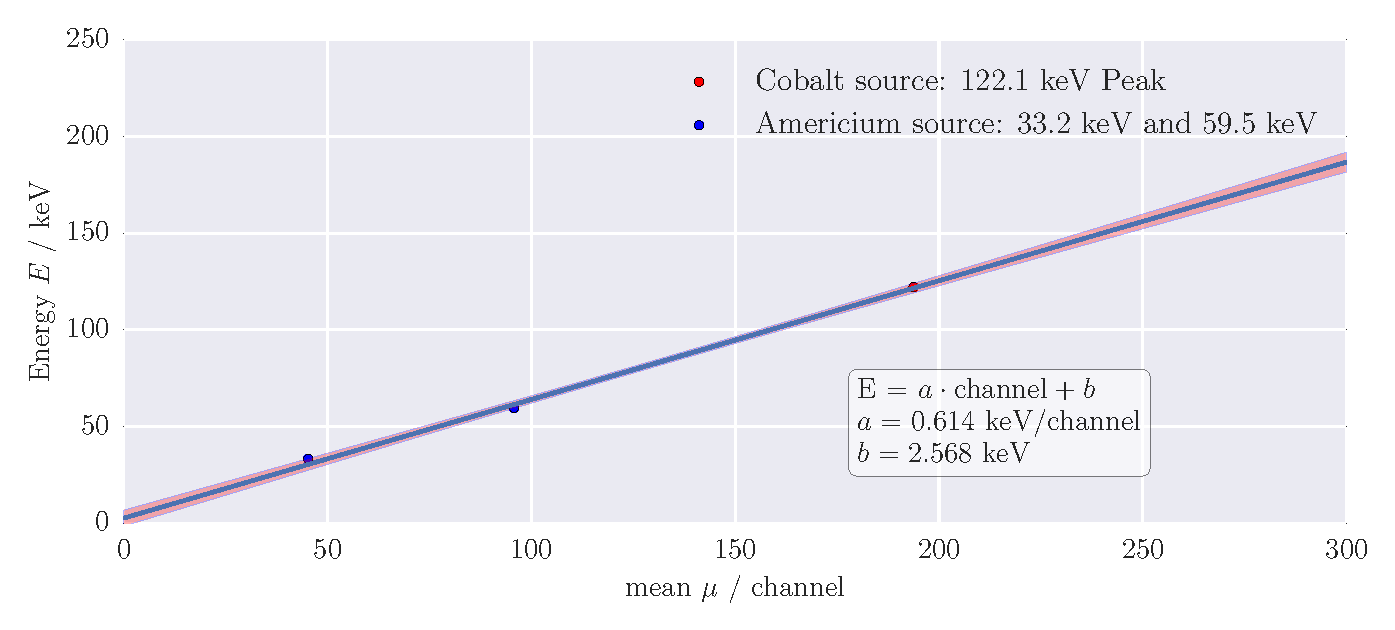
\includegraphics[width=1.0\linewidth]{analysis/figures/plot_E}
    \caption{This is the result of the energy calibration. We used three events about which we were at least
almost sure to have the right events and related them to their respective energy. With three data points  
it definitely does not make sence to use a $\chi^2$-test, so there is no way to check the fidelity.}
    \label{fig:fit_peaks}
\end{figure}

\subsubsection{Calibration of TAC-MCA Signal}
\label{subs:calib_TAC}
In order to relate the channels to the delay, we used the following
measurement for calibration. We used a least square fit for the parameters
of the linear relation:
\begin{align}
    \label{eq:coeff}
    y &= ax + b \\
    a &= \left[ 1.315 \pm 0.005 \right] \mathrm{ns} / \mathrm{Channel}\\
    b &= \left[ -22.6 \pm 0.5 \right]\mathrm{ns} 
\end{align}
where the $x$-values are given by the number of the corresponding channel. 
The resulting covariance matrix of the fit is the following:
\begin{align}
    \label{eq:cov}
    \mathrm{cov}(a, b) &=& 
    \begin{pmatrix}
        2.318 \cdot 10^{-5} &-2.089\cdot 10^{-3}\\
        -2.089\cdot 10^{-3}&2.328\cdot 10^{-1}\\
    \end{pmatrix}
\end{align}
where the units correspond to those of $a$ and $b$ 
(e.~g. $\mathrm{cov}(a,a) = 2.318\mathrm{e}-05 \mathrm{ns^2} / \mathrm{Channel}^2$).
The $\chi^2$-test results in:
\begin{align}
    \label{eq:}
   \chi^2 = 0.972
\end{align}

\label{sub:calibration_of_tac_mca_signal}
\begin{figure}[htpb]
    \centering
    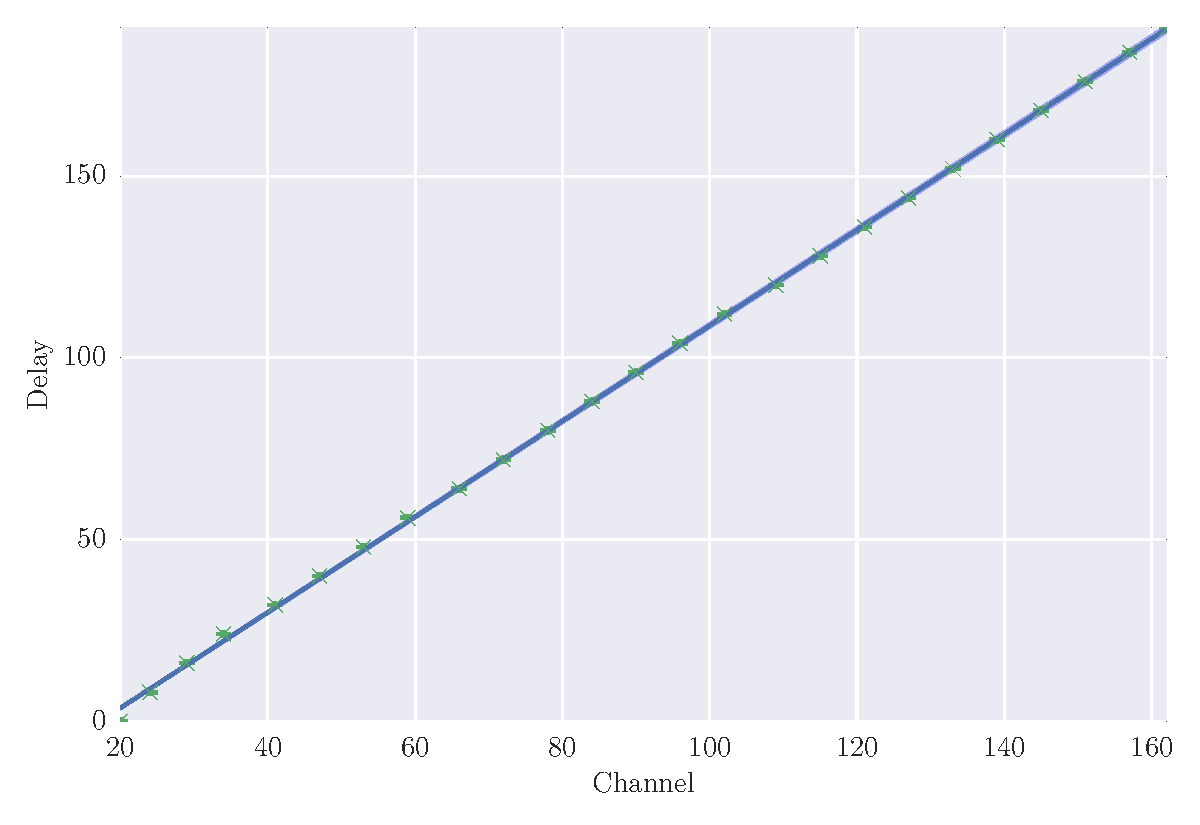
\includegraphics[width=1.0\linewidth]{analysis/figures/plot7}
    \caption{
        Calibration of the TAC-MCA Signal. The errorbars are too small
        to see clearly. Correspondingly, the $\chi^2$ test is almost 1.}
    \label{fig:plot7}
\end{figure}



\subsection{Naive approach: Ad-hoc solution}
In this section we will make use of the previous sections: Forwarding the channel to the time regime and
reducing the background from our main figure in order to evaluate the half life period.\\\\
The measurement of randomized concidences lasted 4.1 lasted \textbf{6080 seconds} = 1 hour 41 minutes and 20 seconds, while
the measurement of delayed coincidences lasted \textbf{52658 seconds} =  14 hours, 37 minutes and 38 seconds. 
In order to compensate for this disparity, we need to extrapolate the background by the following
\begin{equation}
\mathrm{\textbf{total:} } \quad 79 \quad \mathrm{events} \quad \Rightarrow 5.177\cdot 10^{-5}\quad \mathrm{events/ (channel \cdot second)}
\end{equation}
If we extrapolate this for the delayed coincidences, we arrive at
\begin{align}
\begin{split}
\mathrm{\textbf{background estimate:} } \quad  5.177\cdot 10^{-5} \cdot 52658 \quad \mathrm{events / channel} \\
= 2.726\quad \mathrm{events/ channel}
\end{split}
\end{align}
In order to account for the background we will add a constant term to the exponential ansatz (we will already
flip the data in the time regime at the peak in order to reduce the number of freedoms by one):
\begin{equation}
\label{eq:expfit}
a + b\cdot \exp \left [ - \lambda t \right ] 
\end{equation}
It is \textbf{not} feasible to subtract a certain value, for two reasons:
\begin{enumerate}
\item The y-axis corresponds to an integrated number of decays, which is in principle of an poisson distribution,
finding a stable gaussian only for very long measurements. Subtracting a certain value would create \textbf{negative}
events. 
\item If we look more carefully into the distribution of the randomized background, we notice that it is only
in a (in this measurement not realizable) infinite limit equally distributed. We cannot proceed on the assumption
that after 52658s there will be an equally distributed background signal on every channel.
\end{enumerate}
The least squares fit of with \eqref{eq:expfit} results in 

\begin{align}
    \mathrm{cov}&=& 
    \begin{pmatrix}
        0.029 &0.180 &0.000 \\
        0.180 &27.885 &0.009 \\
        0.000 &0.009 &0.000 \\
    \end{pmatrix}
\\ \Rightarrow \qquad
    a &=& 0.07 \pm 0.17 \quad \mathrm{counts}\\
    b &=& 96.6 \pm 5.3 \quad \mathrm{counts}\\
    c &=& 0.0584 \pm 0.0026 \quad \mathrm{ns}^{-1}
\end{align}



\begin{figure}[htpb]
    \centering
    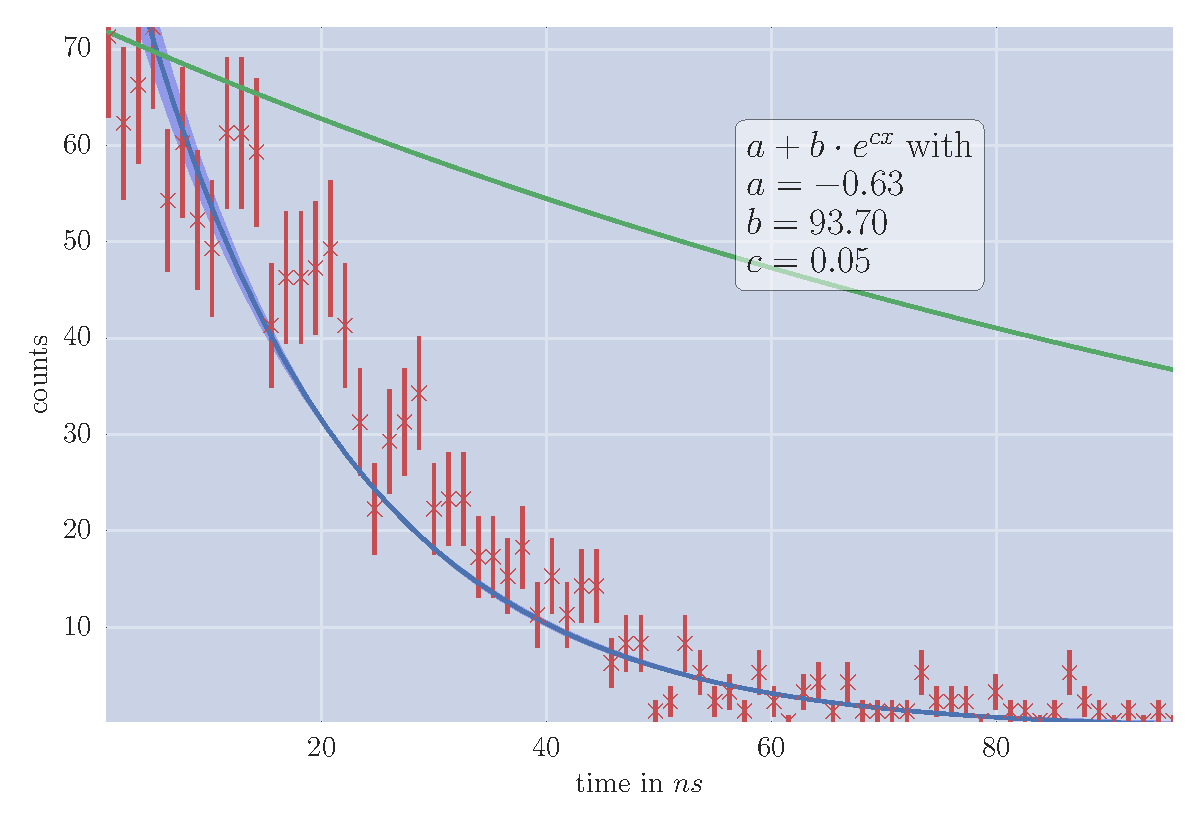
\includegraphics[width=0.8\linewidth]{analysis/figures/plot4_1_reg}
    \caption{This is the result of the exponential fit, where the red bars indicate the measurements with respective
errors whereas the pink line refers to the fit.
The green line indicates the curve with the literature value for $\lambda$ such 
that $N(t) = a + b\cdot e^{-\lambda_{lit} t}$. It is clearly visible that this line does not even agree with
the data at all, neither in the range of their errors nor in their direction. }
    \label{fig:name}
\end{figure}

